
\documentclass{article}
\usepackage{hyperref}
\usepackage{tikz}
\usetikzlibrary{calc}

\usepackage{tikz}
%------------------%
\makeatletter
\newcount\dirtree@lvl
\newcount\dirtree@plvl
\newcount\dirtree@clvl
\def\dirtree@growth{%
  \ifnum\tikznumberofcurrentchild=1\relax
  \global\advance\dirtree@plvl by 1
  \expandafter\xdef\csname dirtree@p@\the\dirtree@plvl\endcsname{\the\dirtree@lvl}
  \fi
  \global\advance\dirtree@lvl by 1\relax
  \dirtree@clvl=\dirtree@lvl
  \advance\dirtree@clvl by -\csname dirtree@p@\the\dirtree@plvl\endcsname
  \pgf@xa=0.5cm\relax % change the length to your needs
  \pgf@ya=-0.75cm\relax % change the length to your needs
  \pgf@ya=\dirtree@clvl\pgf@ya
  \pgftransformshift{\pgfqpoint{\the\pgf@xa}{\the\pgf@ya}}%
  \ifnum\tikznumberofcurrentchild=\tikznumberofchildren
  \global\advance\dirtree@plvl by -1
  \fi
}
\tikzset{ %definition of a new style "dirtree"
  dirtree/.style={
    growth function=\dirtree@growth,
    every node/.style={anchor=north},
    every child node/.style={anchor=west},
    edge from parent path={(\tikzparentnode\tikzparentanchor) |- (\tikzchildnode\tikzchildanchor)}
  }
}
\makeatother


\begin{document}
\tikzset{
    hyperlink node/.style={
        alias=sourcenode,
        append after command={
            let     \p1 = (sourcenode.north west),
                \p2=(sourcenode.south east),
                \n1={\x2-\x1},
                \n2={\y1-\y2} in
            node [inner sep=0pt, outer sep=0pt,anchor=north west,at=(\p1)] {\hyperlink{#1}{\phantom{\rule{\n1}{\n2}}}}
                    %xelatex needs \XeTeXLinkBox, won't create a link unless it
                    %finds text --- rules don't work without \XeTeXLinkBox.
                    %Still builds correctly with pdflatex and lualatex
        }
    }
}

%\hypertarget{pageone}{Page One}
%}


%\tikz \node [draw, inner sep=2ex,hyperlink node=pagetwo] {Go to Page Two};
%\tikz \node (author) at (-2.5,4.1) [draw=black!50,dashed,rectangle,fill=green!20,hyperlink node=pagetwo]{Author}; 

%\tikz \node (reader) at (-2.5, -2.0) [draw=black!50,dashed,rectangle,fill=green!20,hyperlink node=pagetwo] {Go to Page Three};

%     \makebox[.4\textwidth][r]{

%    \makebox[.4\textwidth][l]{
\begin{tikzpicture}[
              outpt/.style={->,blue!80!black,very thick},
              >=stealth,
           every node/.append style={align=center}]
                \node (aux) at (0,18) [draw=black!50,dashed,rectangle,fill=green!30,hyperlink node=pagetwo]{Auxiliary resources}; 
                \node (aux) at (0,17) [draw=black!50,dashed,rectangle,fill=yellow!30,hyperlink node=pagetwo]{Dropbox}; 
  
                \node (measdata) at (-2.4,9) [draw=black!50,dashed,rectangle,fill=orange!30,hyperlink node=proj]{Distributed data}; 
                \node (hypothesis) at (2,9) [draw=black!50,dashed,rectangle,fill=red!30,hyperlink node=pagethree]{Permissions \\ + citations}; 
              \node (anadata) at (0,7.5) [draw=black!50,dashed,rectangle,fill=orange!30] {\begin{tabular}{@{}c}feedback \end{tabular}};
              \node (anadata3) at (0,0) [draw=black!50,dashed,rectangle,fill=orange!30] {\begin{tabular}{@{}c}Version control\end{tabular}};

              \draw[outpt](anadata)--(measdata);
              \draw[outpt](measdata)--(hypothesis);
              \draw[outpt](hypothesis)--(anadata);

  
\end{tikzpicture}
%}
\clearpage
\tikz \node [draw, inner sep=2ex,hyperlink node=pageone] {Main Computer};

\hypertarget{pagetwo}{Page Two}
\clearpage
\hypertarget{pagethree}{Page Three}

\clearpage
\section*{Installation}\label{install}

\subsection*{Data Management Plan}\label{dmp}

\subsection*{Linux}\label{linux}
Some content.

\subsection*{Mac}\label{mac}
Some content.

\subsection*{Windows}\label{win}
Some content.
\clearpage
\section*{Get started}\label{start}
\subsection*{First: Do A}\label{caseA}
Some content.

\subsection*{Second: Do B}\label{caseB}
 Some content.
\clearpage
\section*{Trouble shooting}\label{trbl-shoot}
\subsection*{If X happens:}\label{caseX}
Some content.

\subsection*{If Y happens:}\label{caseY}
 Some content.

\subsection*{Data Inventory}\label{datinv}
\subsection*{Worklog2}\label{mac2}
\subsection*{Worklog}\label{mac3}

Conventions used for writing these entries are:
\begin{quote}
- Names follow this structure [**] [date in ISO 8601] [meeting/notes/results] [from UserName] [Re: topic shortname]
- 'meetings' are for both agenda preparation and also notes of discussion
- 'notes' are such things as emailed information or ad hoc Discovery
- 'results' are entries related to a section of the 'results' folder. 
  That is, this kind of entry is in parallel to the results entry,
  however the log contains a prose description of the experiment,
  whereas the results folder contains scripts etc of all the gory
  details.  
\end{quote}
\subsection*{Workflow}\label{workflow}

\subsection*{Data Provided}\label{dataprov}
\clearpage
\subsection*{Project Management}\label{proj}
\hypertarget{proj}{Project Management stuff}
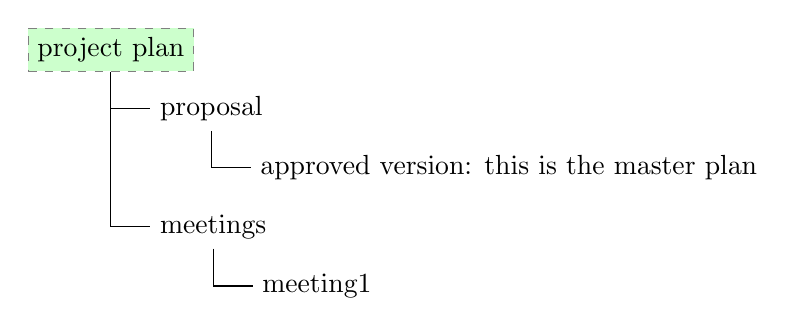
\begin{tikzpicture}[dirtree] % it's what we defined above
  
\node [draw=black!50,dashed,rectangle,fill=green!20]{{project plan} }
      child { node {{proposal} }
          child { node {{approved version: this is the master plan}} }
      }
      child { node {{meetings} }
          child { node {{meeting1}} }
      };

\end{tikzpicture}
\end{document}
